
% report for cs89 final project

\documentclass{article}

\usepackage{subcaption}
\usepackage{fullpage}
\usepackage{listings}
\usepackage{fixltx2e}
\usepackage{graphicx}
\usepackage{dirtree}
\usepackage{caption}
\usepackage{amsmath}
\usepackage{mdwlist}
\usepackage{natbib}
\usepackage{xcolor}
\usepackage{float}

\usepackage{hyperref}

\setlength{\parskip}{3mm}

\begin{document}

\title{Learning the Structure of Local Neural Circuits in Mouse Ectorhinal Cortex}
\author{Scott Brookes and Derek Racine}
\date{May 19, 2014}

\maketitle

%%%%%%%%%%%%%%%%%%%%%%%%%%%%%%%%% INTRODUCTION %%%%%%%%%%%%%%%%%%%%%%%%%%%%%%%%
\section*{Introduction}
The brain is structured such that local networks of neurons can perform 
distinct, modular, tasks. For example, the ectorhinal cortex is known to 
receive the majority of its input from visual sensory areas and is involved 
in visual memory and object recognition. However, the network structure is 
not well understood. Training an animal to recognize certain images, such as 
through visual paired-associate learning, might also affect the network 
dynamics. In particular, one might hypothesize that this training could cause 
neurons to become tuned to images that the mouse has seen before, but not 
others. That is, the activity of neurons would be well correlated with 
stimuli used during training. Yet, this relationship hasn't been 
explored. \par 

Simplified neurons can be described as being in one of two states: resting or 
firing. When a neuron fires, calcium ions flow into it from the extracellular 
fluid. As such, fluorescence observed from calcium sensors can serve as a 
proxy for neural activity. \par

The recent discovery of an ultrasensitive family of fluorescent calcium 
sensors, GCaMP6, has caused an explosion in the availability of time-series 
data based on the use of this technique.\cite{chen13} Whereas previous 
recording methods were limited to only a few cells, fluorescent imaging 
techniques can measure the activity of an entire region of neurons 
simultaneously, as shown in Figure \ref{neurons}. This data offers 
an opportunity to learn the structure of local neural circuits through 
statistical methods. Indeed, previous work has addressed this problem by 
modeling fluorescent imaging data as a collection of coupled Hidden Markov 
chains, one for each neuron.\cite{mishchenko11} \par

\begin{figure}[h]
  \centering
  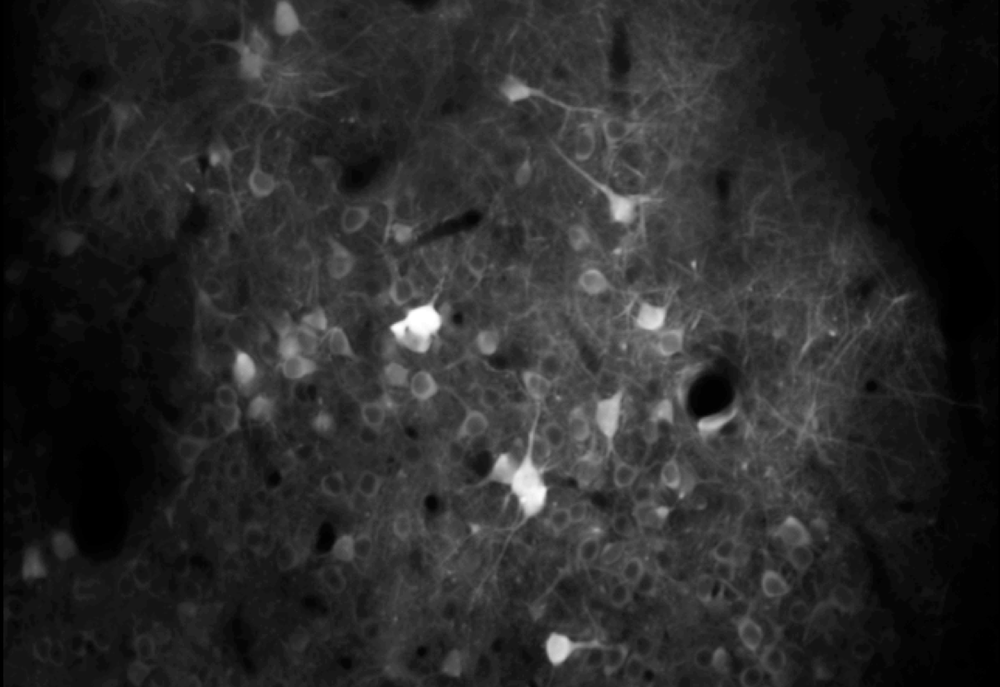
\includegraphics[width=0.5\textwidth]{neurons}
  \caption{A snapshot of neurons labeled with GCaMP6s within a region of the cortex.}
  \label{neurons}
\end{figure}

%%%%%%%%%%%%%%%%%%%%%%%%%%%%%%%%%   DATASET    %%%%%%%%%%%%%%%%%%%%%%%%%%%%%%%%
\section*{Dataset}

We have obtained data sets from the Max Planck Institute for Neurobiology 
corresponding to four recording sessions from the same mouse. Each recording 
session consists of multiple time series of fluorescent activity corresponding 
to the neurons within the imaged area. GCaMP6s, a slower decaying member of 
the GCaMP6 family, was used as the calcium sensor in these experiments. The 
first data set consists of activity of neurons in the primary visual cortex 
(V1) that are known to reliably respond to oriented gratings at a certain 
angle, which are presented to the mouse during the trial. An illustration of 
this setup is shown in Figure \ref{setup}. This data will be a useful control 
for testing our structure learning method because we expect that there will be 
a strong correlation between neural activity and the display of specific 
stimuli. \par

The remaining data sets track the activity of neurons in the ectorhinal cortex 
during periods of spontaneous activity, the display of novel stimuli, and the 
display of these same stimuli after learning to do a visual paired-associate 
task with a subset of them. Inferring both network structure and edge weights 
for these time series will allow us to determine whether neurons become tuned 
to stimuli that the mouse has learned to dscriminate. We also plan on 
investigating the difference between the correlation neurons exhibit during 
spontaneous activity versus when a stimulus is present. \par

\begin{figure}[h]
  \centering
  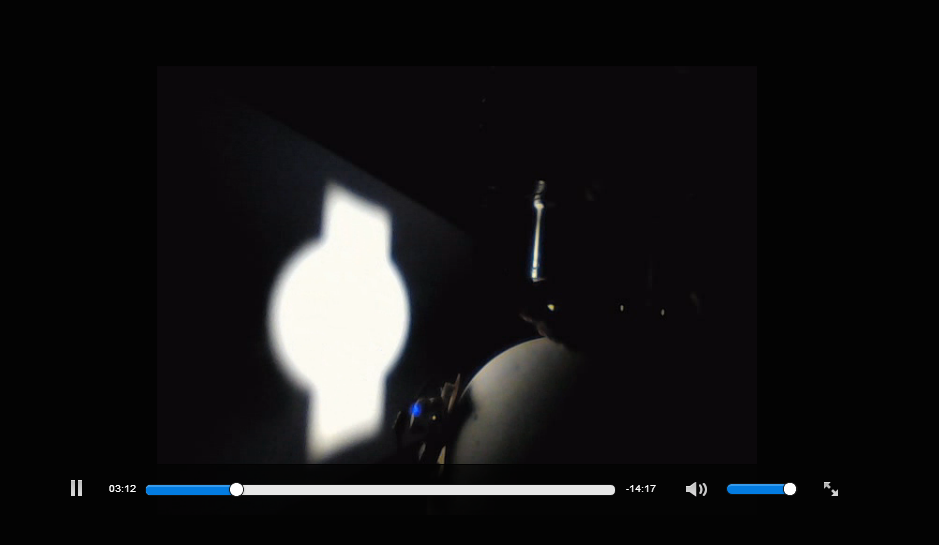
\includegraphics[width=0.5\textwidth]{looming}
  \caption{A photo of the experimental setup in which the mouse is simultaneously viewing a screen where stimuli are presented and being recorded from.}
  \label{setup}
\end{figure}

%%%%%%%%%%%%%%%%%%%%%%%%%%%%%%%%%    METHOD    %%%%%%%%%%%%%%%%%%%%%%%%%%%%%%%%
\section*{Method}

We propose to model the local neural circuits as a Bayesian network and infer 
the edges from the correlations of the activity of individual neurons, which 
we will treat as binary random variables – firing or not firing. In order to 
learn the structure, we plan to discretize our continuous series into buckets 
that each represent a single instance of the overall network. \par

We are using the GlobalMIT toolbox for learning the globaly optimal Dynamic 
Bayes Net structure.\cite{globalmit} The toolbox uses the recently introduced 
\emph{mutual information test (MIT)}. It is implemented in both 
Matlab\textsuperscript{\textregistered} and C++. \par

\subsection*{The Mutual Information Test}

We will present just a brief overview of this method. For a full discussion of 
this algorithm, we direct an interested reader to.\cite{vinh11} \par

A potential network is scored by the total mutual information shared between 
each node and its parents, less a term that quatifies how statistically 
significant the shared information is. The full discussion shows that the 
first term, considering the total mutual information shared between each node 
and its parents, is equivalent to maximizing the log-likelihood criterion. 
As we know, however, learning a Bayes Net using maximum log-likelihood alone 
risks overfitting the data. In order to avoid this unnecessary complexity, the 
MIT method considers whether the information gained by adding a parent to a 
node is statistically significant. This effectively penalizes a complex 
model. \par

\subsection*{Using the Toolkit}

Using the toolkit is rather simple. In order to illustrate the power of the 
toolkit, we give two toy examples that illustrate the output of the toolkit 
given some input. For the output shown in Figure \ref{toy1}, the input is 
a data matrix shown in Figure \ref{tab:toy1} where that table has different 
timeslices as columns and different variables as rows. The same format is used
to display the data table shown in Figure \ref{tab:toy2} used for the toy 2 
example shown in Figure \ref{toy2}. 

\begin{figure}[h]
  \centering
  \begin{tabular}{c |  c | c| c|  c |c| c| c| c| c| c| c| c|c|c|c|c|c|c|c}
    \hline
    1 & 1 & 1 & 1 & 1 & 0 & 0 & 0 & 0 & 0 & 0 & 0 & 0 & 0 & 0 & 0 &0&0&0& 0 \\
    0 & 0 & 0 & 0 & 0 & 1 & 1 & 1 & 1 & 1 & 0 & 0 & 0 & 0 & 0 & 0 &0&0&0& 0 \\
    0 & 0 & 0 & 0 & 0 & 0 & 0 & 0 & 0 & 0 & 1 & 1 & 1 & 1 & 1 & 0 &0&0&0& 0 \\
    0 & 0 & 0& 0 & 0 & 0 & 0 & 0 & 0 & 0 & 0 & 0 & 0 & 0 & 0 & 1 &1&1&1& 1 \\
    \hline
  \end{tabular}
    \caption{Toy1 Dataset}
    \label{tab:toy1}

\end{figure}

\begin{figure}[h]
  \centering
  \begin{tabular}{c| c| c| c| c| c| c| c|c|c|c|c|c|c|c}
    \hline
    1 & 1 & 1 & 1 & 1 & 1 & 1 & 0 & 0 & 0 & 0 & 0 & 0 & 0 & 0 \\
    0 & 0 & 0 & 0 & 0 & 0 & 1 & 1 & 1 & 1 & 1 & 1 & 1 & 1 & 1 \\ 
    0 & 0 & 0 & 0 & 0 & 0 & 1 & 1 & 1 & 1 & 1 & 1 & 1 & 1 & 1 \\ 
    0 & 0 & 0 & 0 & 0 & 0 & 1 & 1 & 1 & 1 & 1 & 1 & 1 & 1 & 1 \\ 
    \hline
  \end{tabular}
    \caption{Toy2 Dataset}
    \label{tab:toy2}

\end{figure}

\begin{figure}[h]
  \centering

  \begin{subfigure}{0.25\textwidth}
    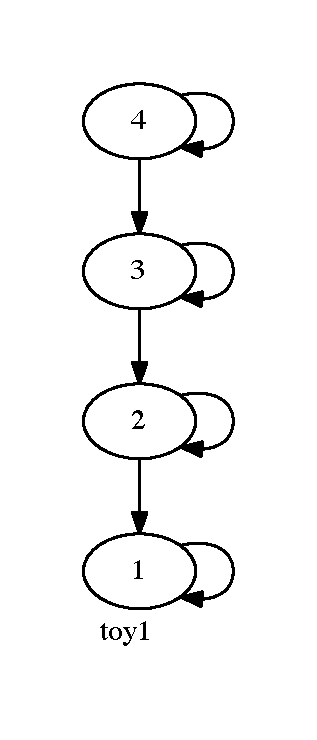
\includegraphics[width=\textwidth]{toy1}
    \subcaption{Toy1 Example Output}
    \label{toy1}
  \end{subfigure}
  ~
  \begin{subfigure}{0.5\textwidth}
    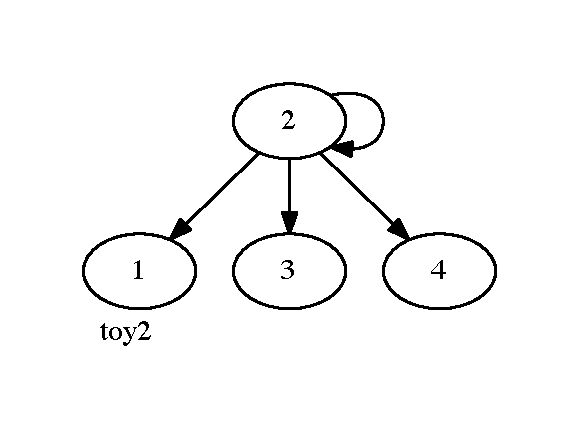
\includegraphics[width=\textwidth]{toy2}
    \subcaption{Toy2 Example Output}
    \label{toy2}
  \end{subfigure}

  \caption{Toy Example Outputs}
  \label{toys}
\end{figure}

\subsection*{Implementation Considerations}

The toolkit takes a parameter $\alpha : 0 < \alpha \le 1$ that tunes the rigor 
to which the algorithm will try to fit the model. Lower $\alpha$'s allow for 
a lower degree of uncertainty, so a lower $\alpha$ generates a more accurate 
result but also requires a great deal more computation time. \par

In order to model the entire neural network that we are interested in, we will 
need to make provisions for minimizing the complexity. The 
paper\cite{globalmit} demonstrates a problem in which there are 20 variables 
and 2,000 observations. In the Matlab\textsuperscript{\textregistered} version 
of the toolkit this model takes more than a full day to be learned. Our 
dataset, naively, has as many as 100 variables with 24,000 observations. \par

In order to achieve practical computation times, we will have to preform data 
preprocessing discussed in other sections of this paper including bucketing to 
get the number of observations down. In addition, the paper discusses that the 
C++ implementation of the toolkit takes only an hour to process this same 
example, leading us to believe that we may need to move towards the C++ 
implementation. This should not require too much effort once we familiarize 
ourselves with the tools on the Matlab\textsuperscript{\textregistered} 
side.\par 

%%%%%%%%%%%%%%%%%%%%%%%%%%%%%%%%%  EVALUATION  %%%%%%%%%%%%%%%%%%%%%%%%%%%%%%%%
\section*{Measuring Success}


We expect that the structure we learn from the first data set will reflect the 
high correlation between neural activity and the presence of particular 
stimuli in V1. After we have verified that this is indeed the case, we will 
apply the same method to the other data sets in order to learn the network 
structure of the neural circuit in the ectorhinal cortex. \par

%%%%%%%%%%%%%%%%%%%%%%%%%%%%%%%%%  CHALLENGES  %%%%%%%%%%%%%%%%%%%%%%%%%%%%%%%%

\section*{Challenges}

Data wrangling has been an enormous time sink. The time series activity is 
extremely noisy, varies independently for each neuron, and includes 
observations when the shutter is closed. As such, the data requires 
significant preprocessing in addition to hand-tweaking, for example, the 
window size considered for smoothing and the threshold for determining when a 
neuron should be considered firing. \par

Structure learning was also complicated by the fact that the data is sparse; 
neurons fire very infrequently throughout the training session.\par

\bibliographystyle{plain}
\bibliography{bibliography}

\end{document}
